% !TeX root = surprises.tex

\selectlanguage{hebrew}

\chapter{פתרון משוואות ריבועיות}\label{c.quadratic}

פרק זה מציג את השיטה לפתרון משוואות ריבועיות של 
\L{Po-Shen Loh}.

\section{השיטות המסורתיות לפתרון משוואות ריבועיות}\label{s.traditional}

כל תלמיד לומד את הנוסחה למצוא את השורשים של משוואה ריבועית
$ax^2+bx+c=0$:
\[
x_1, x_2 = \frac{-b\pm\sqrt{b^2-4ac}}{2a}\,.
\]
נגביל את עצמנו למשוואות שהמקדם הראשון הוא אחד, כי תמיד אפשר לחלק ב-%
$a$.
השורשים של
$x^2+bx+c=0$
הם:
\[
x_1, x_2 = \frac{-b\pm\sqrt{b^2-4c}}{2}\,.
\]
שיטה נוספת היא לפרק את הפולינום הריבועי. לעתים קל לפרק את הפולינום:
\erh{0pt}
\begin{equationarray*}{rcl}
x^2-4x+3& =& (x-r_1)(x-r_2)=0\\
& =& (x-1)(x-3)=0\\
x_1,x_2&=&1, 3\,.
\end{equationarray*}
קשה הרבה יותר לפרק את הפולינום:
\[
x^2-2x-24= (x-r_1)(x-r_2)=0\,.
\]
השורשים האפשריים הם:
\[
(\pm 1,\mp 24)\,, (\pm 2,\mp 12)\,, (\pm 3,\mp 8)\,, (\pm 4,\mp 6)\,.
\]
ברור שהסימנים של
$r_1,r_2$
שונים כי המכפלה שלילית
$-24$,
אבל עדיין יש לבדוק שמונה אפשרויות.



\section{חישוב השורשים}\label{s.computing}

\textbf{אם}
$r_1,r_2$
\textbf{הם השורשים של}
$x^2+bx+c$,
אזי:%
\footnote{%
\L{Loh}
מדגיש את ההבדל בין שיטתו לבין פירוק. בפירוק, אני 
\textbf{מניחים}
שקיימים שני שורשים. ההנחה נכונה לפי המשפט הבסיסי של אלגברה, אבל זה משפט "כבד" עבור המשימה הפשוטה של מציאת שורשים של משוואה ריבועית. לפי שיטתו, אנחנו רק אומרים:
\textbf{אם השורשים קיימים}.%
}
\[
(x-r_1)(x-r_2)=x^2 - (r_1+r_2)x + r_1r_2=x^2+bx+c\,.
\]
אפילו אם אין אנו יודעים את ערכי השורשים, אנו כן יודעים ש:
\[
r_1+r_2 = -b\,,\quad\quad r_1r_2=c\,.
\]
נסתכל על מספר ערכים עבור
$-b,r_1,r_2$
ונסמן ב-%
$m_{12}$
את הממוצע של
$r_1,r_2$:
\[
\renewcommand{\arraystretch}{1.3}
\begin{array}{|r|r|r|r|}
\hline
-b& r_1 & r_2 &m_{12}\\\hline
\hline
33 & 12 & 21 & 16\frac{1}{2}\\\hline
33 & 8 & 25 & 16\frac{1}{2}\\\hline
33 & 1 & 32 & 16\frac{1}{2}\\\hline
\hline
-4 & -16 & 12 & -2 \\\hline
-4 & -4 & 0 & -2 \\\hline
-4 & -3 & -1 & -2 \\\hline
\end{array}
\]
עבור כל משוואה ריבועית, הממוצע של שני השורשים קבוע:
\[
\frac{r_1+r_2}{2}=
\frac{(-b-r_2)+r_2}{2}=
\frac{-b}{2}+\frac{-r_2+r_2}{2}=
-\frac{b}{2}\,.
\]
יהי 
$s$ 
מספר כלשהו, אזי:
\[
-b=-b+s+(-s)=\left(\frac{-b}{2}+s\right) + \left(\frac{-b}{2}-s\right)=r_1+r_2\,.
\]
אם שורש אחד נמצא במרחק
$s$
מהממוצע, השורש השני נמצא במרחק
$-s$
מהממוצע:
\[
\renewcommand{\arraystretch}{1.3}
\begin{array}{|r|r|r|r|r|r|}
\hline
-b& r_1 & r_2 & m_{12}& m_{12}-r_1 & m_{12}-r_2\\\hline\hline
33 & 12 & 21 & 16\frac{1}{2}&4\frac{1}{2} & -4\frac{1}{2}  \\\hline
33 & 8 & 25 & 16\frac{1}{2}&8\frac{1}{2}&-8\frac{1}{2}\\\hline
33 & 1 & 32 & 16\frac{1}{2}&15\frac{1}{2}&-15\frac{1}{2}\\\hline
\hline
-4 & -16 & 12 & -2 &14& -14\\\hline
-4 & -4 & 0 & -2&2&-2 \\\hline
-4 & -3 & -1 & -2&1&-1 \\\hline
\end{array}
\]

\bigskip

התרשים שלהלן מראה את היחסים הללו עבור
$r_1,r_2=2,6$,
כאשר
$m_{12}=4, s=2$:
\selectlanguage{english}
\begin{center}
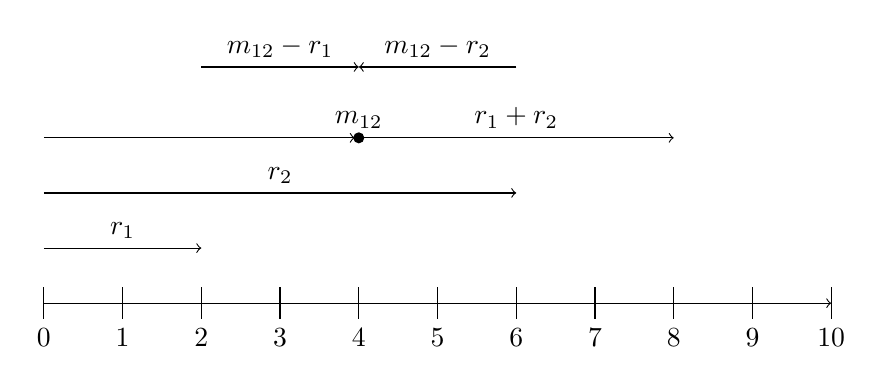
\begin{tikzpicture}
\draw[->] (0,0) -- (10,0);
\foreach \x in {0,1,...,10}
  \draw (\x,-2mm) -- +(0,4mm) node[below,yshift=-4mm] {$\x$};
\draw[->,yshift=7mm] (0,0) -- node[above] {$r_1$} (20mm,0);
\draw[->,yshift=14mm] (0,0) -- node[above] {$r_2$} (60mm,0);
\draw[->,yshift=21mm] (0,0) -- (39.5mm,0);
\draw[->,yshift=21mm] (40mm,0) -- node[above] {$r_1+r_2$} (80mm,0);
\fill (40mm,21mm) circle(2pt) node[above] {$m_{12}$};
\draw[->,yshift=30mm] (20mm,0mm) -- node[above] {$m_{12}-r_1$} +(20mm,0);
\draw[->,yshift=30mm] (60mm,0mm) -- node[above] {$m_{12}-r_2$} +(-20mm,0);
\end{tikzpicture}
\end{center}
\selectlanguage{hebrew}
אם נבחר ערכים אחרים
$r_1,r_2=3,5$
עבורם
$r_1+r_2=8$, $m_{12}=4$ 
נשאר ללא שינוי, אבל
$s=1$
משתנה:
\selectlanguage{english}
\begin{center}
\begin{tikzpicture}
\draw[->] (0,0) -- (10,0);
\foreach \x in {0,1,...,10}
  \draw (\x,-2mm) -- +(0,4mm) node[below,yshift=-4mm] {$\x$};
\draw[->,yshift=7mm] (0,0) -- node[above] {$r_1$} (30mm,0);
\draw[->,yshift=14mm] (0,0) -- node[above] {$r_2$} (50mm,0);
\draw[->,yshift=21mm] (0,0) -- (39.5mm,0);
\draw[->,yshift=21mm] (40mm,0) -- node[above] {$r_1+r_2$} (80mm,0);
\fill (40mm,21mm) circle(2pt) node[above] {$m_{12}$};
\draw[->,yshift=30mm] (30mm,0mm) -- node[above left] {$m_{12}-r_1$} +(10mm,0);
\draw[->,yshift=30mm] (50mm,0mm) -- node[above right] {$m_{12}-r_2$} +(-10mm,0);
\end{tikzpicture}
\end{center}
\selectlanguage{hebrew}

לכאורה ההפרש
$s$
שרירותי ב:
\[
r_1=\left(\frac{-b}{2}+s\right)\,,\quad r_2=\left(\frac{-b}{2}-s\right)\,,
\]
אבל קיים אילוץ נוסף
$r_1r_2=c$
כאשר
$c$
הוא הקבוע בפולינום. אם נכפיל את שני ביטויים במצאנו עבור
$r_1,r_2$,
נוכל לחשב את
$s$
ואחר כך את
$r_1,r_2$.
\[
c=\left(-\frac{b}{2} +s\right)\left(-\frac{b}{2} -s\right)\,.
\]


\section{דוגמאות}\label{s.examples}

נשמתש בשיטה על הפולינום
$x^2-2x-24$,
כאשר
$b=-2,c=-24$:
\erh{4pt}
\begin{equationarray*}{rcl}
c&=&\left(-\frac{b}{2} +s\right)\left(-\frac{b}{2} -s\right)\\
-24&=&(1 +s)(1 -s)\\
s^2&=&25\\
s&=&5\\
r_1&=&1+5=6\\
r_2&=&1-5=-4\,.
\end{equationarray*}
נבדוק:
\[
(x-6)(x-(-4))=x^2-6x-(-4)x+(6\cdot -4)= x^2-2x-24\,.
\]
כדוגמה נוספת נמצא את השורשים של
$x^2-83x-2310$:
\erh{12pt}
\begin{equationarray*}{rcl}
c&=&\left(-\frac{b}{2} +s\right)\left(-\frac{b}{2} -s\right)\\
-2310&=&\left(\frac{83}{2}+s\right)\left(\frac{83}{2} -s\right)\\
s^2&=&\frac{6889}{4}+2310=\frac{16129}{4}\\
s&=&\frac{127}{2}\\
r_1&=&\frac{83}{2}-\frac{127}{2}=-22\\
r_2&=&\frac{83}{2}+\frac{127}{2}=105\,.
\end{equationarray*}
נבדוק:
\[
(x+22)(x-105)=x^2+22x-105x+(22\cdot -105)= x^2-83x-2310\,.
\]
נשווה את החישוב עם החישוב המשתמש בנוסחה:
\erh{8pt}
\begin{equationarray*}{rcl}
\frac{-b\pm\sqrt{b^2-4c}}{2}&=&\frac{-(-83)\pm\sqrt{(-83)^2-4\cdot (-2310)}}{2}\\
&=& \frac{83\pm\sqrt{6889+9240}}{2} = \frac{83\pm\sqrt{16129}}{2}\\
&=& \frac{83\pm 127}{2}\\
r_1&=&\frac{83-127}{2}=-22\\
r_2&=&\frac{83+127}{2}=105\,.
\end{equationarray*}
למרות שהחישוב בשיטה של
\L{Loh}
דומה לחישוב עם הנוסחה, יש לה יתרון כי ניתן לקבל את החישוב מיידית מהממוצע ומהמכפלה של השורשים. בסעיף הבא נראה שקל לקבל את הנוסחה המסורתית משיטה זו.

\section{הנוסחה המסורתית}\label{s.general}

עם מקדמים שרירותיים הנוסחאות לפי השיטה של
\L{Loh}
הן:
\erh{12pt}
\begin{equationarray*}{rcl}
c=r_1,r_2&=&\left(\frac{-b}{2}+s\right)  \left(\frac{-b}{2}-s\right)\\
&=&\left(\frac{b^2}{4}-s^2\right)\\
s&=&\sqrt{\left(\frac{b^2}{4}\right)-c}\\
r_1,r_2&=&\frac{-b}{2}\pm\sqrt{\left(\frac{b^2}{4}\right)-c}\\
r_1,r_2&=&\frac{-b\pm\sqrt{b^2-4c}}{2}\,,
\end{equationarray*}
הנוסחה המסורתית לקבלת השורשים של פולינום עם מקדם אחד עבור
$x^2$.

עבור פולינום עם
$a\neq 1$, 
חלקו את המקדמים ב-%
$a$,
הציבו במשוואה ופשטו:
\erh{12pt}
\begin{equationarray*}{rcl}
%ax^2+bx+c&=&0\\
x^2+\frac{b}{a}x+\frac{c}{a}&=&0\\
r_1,r_2&=&\frac{-(b/a)\pm\sqrt{(b/a)^2-4(c/a)}}{2}\\
%&=&\frac{-(b/a)\pm\sqrt{(b/a)^2-4(ac/a^2)}}{2}\\
&=&\frac{-b\pm\sqrt{b^2-4ac}}{2a}\,.
\end{equationarray*}

\section{פולינומים עם שורשים דמיוניים}\label{s.irreducible}

נבדוק את שיטה עבור
$x^2-2x+76$:
\erh{4pt}
\begin{equationarray*}{rcl}
s^2&=&\frac{b^2}{4}-c=\frac{4}{4}-76=-75\\
s&=&\sqrt{-75}=\sqrt{-1\cdot 25\cdot 3}=i\,5\sqrt{3}\\
r_1,r_2&=&1\pm i\,5\sqrt{3}\,.
\end{equationarray*}
נבדוק:
\[
\renewcommand*{\arraystretch}{1}
\begin{array}{ll}
(x-(1+i\,5\sqrt{3}))\;(x-(1-i\,5\sqrt{3}))&=\\
x^2 \,-\, (1+i\,5\sqrt{3})x\,-\,(1-i\,5\sqrt{3})x\,+\,(1^2-(i\,5\sqrt{3})^2)&=\\
%x^2 -x -x + 1 - (-75)&=\\
x^2-2x+76\,.
\end{array}
\]

\subsection*{מקורות}

הפרק מבוסס על
\L{\cite{loh1,loh2}}.


